% ===================================================================
% CHAPTER 4: Sensitivity Analysis of the V2G System
% ===================================================================
\chapter{Sensitivity Analysis of the V2G System}
\label{chap:sensitivity_analysis}


The performance of a Vehicle-to-Grid (V2G) system is governed by a complex interplay of physical, economic, and behavioral parameters. Understanding which of these parameters have the most significant impact on system outcomes is crucial for designing robust and effective control strategies. A controller optimized for one specific set of conditions may perform poorly under slightly different circumstances. Sensitivity Analysis (SA) is a systematic methodology used to quantify how the variation in the inputs of a model influences the variation in its outputs.
\noindent
This chapter presents a comprehensive sensitivity analysis of the EV2Gym simulation environment. The primary objectives are:
\begin{itemize}
    \item To identify the most critical parameters that drive system performance, particularly economic profitability and grid stability.
    \item To understand how different control algorithms (heuristics, MPC, and RL) respond to variations in these parameters.
    \item To gain insights that can guide the development of more robust and generalist control agents.
\end{itemize}
\noindent
The analysis was conducted using the custom-built \textbf{sensitivity\_analysis.py} script,
\\
\noindent which automates the process of running large batches of simulations while systematically varying key input parameters.


\section{Introduction to Global Sensitivity Analysis}

In these sessions, the topic of global sensitivity analysis is discussed, which is presented as a very important method in uncertainty quantification.\noindent
 This method allows for a better understanding of the relationship between data, model, and prediction. There are many techniques for performing such global sensitivity analysis. However, before covering global sensitivity analysis, the speaker first discusses local sensitivity analysis.
\\
\noindent
Sensitivity analysis is defined as a study where uncertain input parameters are varied to understand how that variation results in a change in some response of interest. This response of interest can be anything, such as a data variable or a prediction variable.
\\
\noindent
SA is the study of how variation of uncertain input parameters impacts the uncertainty of the response of interest.
\noindent
\textit{Note: There is no unique way of doing sensitivity analysis.}
\\
\noindent
In this context, sensitivity analysis allows for the reduction of uncertainty in predictions, as it facilitates the identification of input parameters that affect those predictions. This, in turn, can help identify what data needs to be acquired to reduce uncertainty on those parameters.

\begin{itemize}
    \item \textbf{SA can aid in reducing uncertainty in prediction} by identifying high-impact parameters. This can indicate which data to acquire to reduce uncertainty on said parameters.
    \item \textbf{SA can indicate which parameters have little influence on the prediction.} This may help in reducing the complexity of the problem by either removing those parameters or setting those with little influence to some fixed value.
    \item \textbf{SA can help in quantifying and understanding how the combined effect of parameters generates non-linear variations in responses (interactions).} When dealing with nonlinear systems or functions, as is common in uncertainty quantification problems and the forward models used, these nonlinear variations in responses are frequent. In such systems, a phenomenon known as "interactions" occurs. This concept will be covered in great detail.
\end{itemize}
\noindent
As a side note, it is mentioned that there is no single, unique way of performing sensitivity analysis. Therefore, referring to "the" sensitivity analysis would actually point to a specific method. Each method allows for the study of different aspects, and it is important to understand which method is suitable for a given situation and application.


\section{Different Classes of Sensitivity Analysis}

There are many different classes of sensitivity analysis, but for the purposes of this course, the discussion focuses on local sensitivity analysis and global sensitivity analysis.

\subsection{Local SA}
In local sensitivity analysis, the process starts from a base case. This could be the mean of the parameters, or a single model can be built based on the available information. Once such a model or base case is established, the effect of making perturbations to that model is evaluated. Perturbations can be implemented in various ways; for instance, one can calculate the partial derivatives of the forward response function, given that the analysis is in the base case scenario. It is also possible to have multiple base case scenarios and evaluate sensitivity on each of them.

\begin{itemize}
    \item Evaluates sensitivity for a single (deterministic) set of input parameters.
    \item Often based on partial derivatives of the response with respect to the parameters. The sensitivity measure is only informative for the particular set of parameters.
    \item Fast to compute ($N_p + 1$ model evaluations).
\end{itemize}
\begin{algorithm}[H]
\caption{Local Sensitivity Analysis (LSA)}
\begin{algorithmic}[1]
\State \textbf{Input:} model $f(\mathbf{x})$ with parameters $\mathbf{x} = [x_1, x_2, \dots, x_{N_p}]$, base case $\mathbf{x}_0$
\State \textbf{Output:} local sensitivity $S_i$ for each parameter $x_i$
\State Build the base model: $y_0 = f(\mathbf{x}_0)$
\For{$i = 1$ to $N_p$}
\State Perturb parameter $i$ by a small $\Delta x_i$: $\mathbf{x}_i^+ = \mathbf{x}_0 + \Delta x_i \mathbf{e}_i$ 
\State Calculate the answer: $y_i^+ = f(\mathbf{x}_i^+)$ 
\State Calculate the local sensitivity: 
\[ 
S_i = \frac{y_i^+ - y_0}{\Delta x_i} \approx \frac{\partial f}{\partial x_i} \Big|_{\mathbf{x}_0} 
\]
\EndFor
\State \textbf{Return:} $S_1, S_2, \dots, S_{N_p}$
\end{algorithmic}
\end{algorithm}

\subsection{Global SA (GSA)}
In global sensitivity analysis, the base case scenario is disregarded. Instead, a Monte Carlo simulation is performed on the input parameters. The model is run many times with various input parameters drawn from a prior distribution. The models are then evaluated to understand the multivariate distribution of the output that is generated due to the variation of the input parameters.

\begin{itemize}
    \item Assesses the effect of large changes in the input parameters, which is more appropriate for uncertainty quantification.
    \item Requires many model evaluations.
\end{itemize}

\section{Challenges}
The challenges (very common in geosciences) or uncertainty quantification are:
\begin{itemize}
    \item \textbf{High dimensional problem:}
    \begin{itemize}
        \item Many uncertain input parameters.
        \item Response may be high dimensional.
    \end{itemize}
    \item \textbf{Large computational time:} Evaluating responses such as forward models and making predictions involves large computational times.
    \item \textbf{Non-linearity of the models:} The non-linearity of the problem is quite substantial.
    \item \textbf{Spatial aspect of the models:} There is a spatial aspect, such as the spatial distribution of hydraulic conductivity, permeability, porosity, or layering, which needs to be taken into account as it may have a considerable influence on the response. The problem is how to quantify the influence of spatial variability (which is not a simple variable) on some kind of response.
\end{itemize}

\section*{Screening Techniques}
Two techniques are introduced: one-at-a-time (OAT) analysis and the Morris method. Both are simplified approaches. They are quite useful for "screening" because they require only a small number of model evaluations. However, it is very difficult to draw general conclusions from these methods, as there are several drawbacks when applying them to the kind of problems being addressed.
\subsection*{Algorithmic Description of OAT and Morris Methods}

\begin{algorithm}[H]
\caption{One-at-a-Time (OAT) Sensitivity Analysis}
\begin{algorithmic}[1]
\State \textbf{Input:} model $f(\mathbf{x})$ with parameters $\mathbf{x} = [x_1, \dots, x_{N_p}]$, base case $\mathbf{x}_0$, perturbation factor $\Delta$
\State \textbf{Output:} parameter influence ranking
\State Evaluate the base case: $y_0 = f(\mathbf{x}_0)$
\For{$i = 1$ to $N_p$}
    \State Perturb the $i$-th parameter: $\mathbf{x}_i^+ = \mathbf{x}_0 + \Delta x_i \mathbf{e}_i$
    \State Evaluate the model: $y_i^+ = f(\mathbf{x}_i^+)$
    \State Compute the effect of parameter $i$: $S_i = y_i^+ - y_0$
\EndFor
\State Rank parameters based on $|S_i|$ to determine their influence
\State \textbf{Note:} Requires $2 \times N_p + 1$ model evaluations for full analysis.
\end{algorithmic}
\end{algorithm}

\begin{algorithm}[H]
\caption{Morris Method (Elementary Effects Method)}
\begin{algorithmic}[1]
\State \textbf{Input:} model $f(\mathbf{x})$ with parameters $\mathbf{x} = [x_1, \dots, x_{N_p}]$, number of trajectories $L$, perturbation $\Delta$
\State \textbf{Output:} $\mu_n^*$, $\sigma_n$ for each parameter
\For{$l = 1$ to $L$} 
    \State Generate a random starting point $\mathbf{x}^{(l)}$ in the parameter space
    \For{$n = 1$ to $N_p$}
        \State Perturb parameter $n$: $\mathbf{x}^{(l)}_n = \mathbf{x}^{(l)} + \Delta \mathbf{e}_n$
        \State Compute the elementary effect: 
        \[
        EE_n^{(l)} = \frac{f(\mathbf{x}^{(l)}_n) - f(\mathbf{x}^{(l)})}{\Delta}
        \]
    \EndFor
\EndFor
\For{$n = 1$ to $N_p$}
    \State Compute mean of absolute elementary effects:
    \[
    \mu_n^* = \frac{1}{L} \sum_{l=1}^{L} |EE_n^{(l)}|
    \]
    \State Compute standard deviation of elementary effects:
    \[
    \sigma_n = \sqrt{\frac{1}{L-1} \sum_{l=1}^{L} (EE_n^{(l)} - \bar{EE}_n)^2}
    \]
\EndFor
\State \textbf{Interpretation:} Plot $\sigma_n$ vs $\mu_n^*$ to classify parameters:
\begin{itemize}
    \item Negligible effects: small $\mu_n^*$ and small $\sigma_n$
    \item Linear and additive effects: large $\mu_n^*$ and small $\sigma_n$
    \item Non-linear or interaction effects: large $\mu_n^*$ and large $\sigma_n$
\end{itemize}
\end{algorithmic}
\end{algorithm}

\section*{Note on Interactions}
Interactions are an often poorly understood concept. An example is given where a material (e.g., shale rock) is tested, and its strength (response Z) is evaluated based on two factors: temperature (X) and composition ratio (Y). A factorial design can be set up with high and low levels for each factor.
\noindent
An interaction means that the effect of one factor depends on the level of another factor. The main effects of X and Y, as well as the interaction effect XY, can be estimated. In many cases, the interaction effect (the combined effect of temperature and composition) can be the most significant factor, more so than either factor individually. This indicates a non-linear relationship where the whole is greater than the sum of its parts.

\subsection*{Digest of Screening Techniques}
\begin{itemize}
    \item Rapidly gives insight into parameter influence with a small number of model evaluations.
    \item Only provides qualitative/subjective measures of sensitivity.
    \item Does not evaluate or distinguish interactions from non-linear effects well.
    \item Requires only a single response.
    \item Cannot be applied to non-numerical input (e.g., scenarios).
    \item Requires continuity in the response, which means it cannot be applied with spatial uncertainty.
    \item As a precursor to GSA, the Morris method may identify parameters that can be removed from the study, simplifying the problem.
\end{itemize}


\section{Methodology for Sensitivity and Robustness Analysis}
\label{sec:sa_methodology}
\noindent
To systematically investigate the V2G system's behavior and train robust control agents, this work employs a suite of increasingly sophisticated methodologies, all orchestrated through the \textbf{sensitivity\_analysis.py} and \textbf{run\_interactive.py} scripts. These methods range from classical sensitivity analysis techniques to advanced, dynamic training environments.

\subsection{Parameter and Model-Output Space}
\noindent
The foundation for all analysis is a defined set of input parameters and output metrics. The input space consists of nine key parameters identified as having a potentially high impact on the system's operation. For each parameter, a set of discrete, realistic levels was established, as detailed in Table \ref{tab:sa_parameters_detailed}. The primary output metric, or Key Performance Indicator (KPI), used for evaluating sensitivity is the \textbf{Total Profit (€)} generated by a control agent over a full simulation run.

\begin{table}[H]
    \centering
    \caption{Parameters and Levels for Sensitivity Analysis}
    \label{tab:sa_parameters_detailed}
    \begin{tabular}{|l|l|l|}
        \hline
        \textbf{Parameter} & \textbf{Baseline} & \textbf{Levels} \\ \hline
        Number of Charging Stations & 25 & 5, 15, 25, 50, 100 \\ \hline
        Transformer Max Power (kW) & 100 & 25, 50, 100, 200, 400 \\ \hline
        EV Spawn Multiplier & 5 & 1, 3, 5, 7, 10 \\ \hline
        EV Charge Efficiency & 0.95 & 0.80, 0.90, 0.95, 0.99 \\ \hline
        EV Discharge Efficiency & 0.90 & 0.70, 0.85, 0.90, 0.98 \\ \hline
        EV Desired Capacity (\%) & 1.0 & 0.6, 0.75, 0.85, 0.95, 1.0 \\ \hline
        Discharge Price Factor & 1.0 & 0.5, 0.8, 1.0, 1.5, 2.0 \\ \hline
        Inflexible Loads Forecast Mean & 30\% & 0, 15, 30, 45, 60 \\ \hline
        Solar Power Forecast Mean & 20\% & 0, 20, 40, 60, 80 \\ \hline
    \end{tabular}
\end{table}

\subsection{One-at-a-Time (OaaT) Sensitivity Analysis}
\noindent
The OaaT method is the most fundamental approach to sensitivity analysis. It operates by varying a single input parameter across its predefined levels while keeping all other parameters fixed at their baseline values. For example, to analyze the impact of the transformer capacity, simulations are run with the `Transformer Max Power (kW)` set to 25, 50, 100, 200, and 400, while the other eight parameters remain unchanged.
\noindent
The primary advantage of OaaT is its simplicity and the clarity of its results. It produces easy-to-interpret graphs showing the direct relationship between one input and one output. However, its major drawback is that it cannot detect interactions between parameters. The effect of changing the transformer power might be very different when the `EV Spawn Multiplier` is high compared to when it is low, and OaaT cannot capture this type of synergistic effect.

\subsection{Global Sensitivity Analysis: The Morris Method}
\noindent
To overcome the limitations of OaaT, we employ the Morris method, a global sensitivity analysis technique proposed by Max D. Morris in 1991 for efficient parameter screening. It is a "one-at-a-time" method, but it is executed at many different points in the input parameter space, and the results are then averaged.

\noindent
The sampling process is organized into \textbf{trajectories}, where each trajectory represents a path through the high-dimensional input space. A key implementation choice is the use of \textbf{Optimal Trajectories}, a sophisticated sampling strategy designed to overcome the potential biases of purely random sampling.

\noindent
The concept is analogous to surveying a large area: instead of taking random paths, which might accidentally cluster in one region and miss others entirely, an optimal approach involves pre-planning the paths to ensure the entire area is covered as uniformly as possible. In the context of the Morris method, `SALib` selects a set of trajectories that are maximally "spread out" from each other. This ensures that the elementary effects are calculated in highly diverse regions of the parameter space (e.g., under conditions of both high and low solar power, high and low electricity prices, etc.). By guaranteeing a more systematic and uniform exploration, this optimal sampling strategy produces more robust and reliable sensitivity indices ($\mu^*$ and $\sigma$) for a given number of simulations, reducing the risk of drawing conclusions from an unrepresentative sample of the model's behavior.

\noindent
The core of the method is the calculation of "elementary effects." For a given input parameter $X_i$, an elementary effect is the finite difference in the model output $Y$ when $X_i$ is perturbed by a fixed amount $\Delta$, while all other inputs $X_j$ ($j \neq i$) are held constant.
\begin{equation}
    EE_i(\mathbf{X}) = \frac{Y(X_1, ..., X_i + \Delta, ..., X_k) - Y(\mathbf{X})}{\Delta}
\end{equation}
\noindent
The Morris method generates $r$ different trajectories through the $k$-dimensional input space. For each trajectory, it computes the elementary effect for every parameter. The final output is a set of sensitivity indices for each parameter, derived from the distribution of these elementary effects:
\begin{itemize}
    \item $\mu^*$ (\textbf{mu-star}): The mean of the absolute values of the elementary effects. It is a measure of the parameter's overall influence on the output. A high $\mu^*$ indicates an important parameter.
    \item $\sigma$ (\textbf{sigma}): The standard deviation of the elementary effects. It measures the extent of non-linear effects or interactions with other parameters. A high $\sigma$ suggests that the parameter's effect is not constant but depends on the values of other parameters in the model.
\end{itemize}
\noindent
By plotting $\sigma$ versus $\mu^*$, we can visually classify parameters as either (a) having a large overall effect (high $\mu^*$), (b) being involved in significant interactions (high $\sigma$), or (c) being relatively non-influential (low $\mu^*$ and $\sigma$). This provides a global perspective on the model's sensitivities.

\subsubsection{Implementation with SALib}
To conduct the global sensitivity analysis using the Morris method, the Python library \textbf{SALib} was utilized. The process implemented in the
\\
\noindent
 \textbf{sensitivity\_analysis.py} script can be broken down into the following key steps:

\begin{enumerate}
    \item \textbf{Problem Definition:}
    First, the sensitivity problem is defined. This is done by creating a Python dictionary that specifies the parameters to be analyzed, their names, and their bounds. 
\\
\noindent
This data structure, named \textbf{problem}, is a fundamental requirement for the \textbf{SALib} library.
    
    \begin{verbatim}
problem = {
    'num_vars': len(selected_param_names),
    'names': selected_param_names,
    'bounds': [[min_val_1, max_val_1],
               [min_val_2, max_val_2],
               ...]
}
    \end{verbatim}

    \item \textbf{Sampling:}
    Next, the Morris sampler provided by \textbf{SALib} is used to generate the input points to be evaluated.
\\
\noindent
 The function \textbf{morris\_sampler.sample()} takes the \textbf{problem} dictionary, the number of trajectories to generate (\textbf{N}), and the number of grid levels (\textbf{num\_levels}) as input.
\\
\noindent
 The function returns a NumPy array, \textbf{param\_values}, where each row represents a combination of input parameters on which to run the model.
    
    \begin{verbatim}
from SALib.sample import morris as morris_sampler

param_values = morris_sampler.sample(problem, 
                                     N=num_trajectories, 
                                     num_levels=num_levels)
    \end{verbatim}

    \item \textbf{Model Execution:}
    The code then iterates over each row of the \textbf{param\_values} array. 
\\\noindent
For each combination of parameters, a model simulation is executed (\textbf{run\_benchmark}), and the output of interest (e.g., \textbf{total\_profits}) is recorded. These results are stored in a NumPy array \textbf{Y}.

    \item \textbf{Analysis of Results:}
\noindent
    Once the model has been run for all sampling points, the results are analyzed using the \textbf{morris\_analyzer.analyze()} function. This function calculates the Morris sensitivity indices, primarily:
    \begin{itemize}
        \item \textbf{$\mu^*$ (mu\_star):} An estimate of the mean absolute effect of a parameter on the output. A high value indicates an influential parameter.
        \item \textbf{$\sigma$ (sigma):} The standard deviation of the elementary effects, which indicates non-linear effects or interactions with other parameters.
    \end{itemize}
    
    \begin{verbatim}
from SALib.analyze import morris as morris_analyzer

Si = morris_analyzer.analyze(problem, 
                             param_values, 
                             Y, 
                             conf_level=0.95)
    \end{verbatim}
    
    The returned \textbf{Si} object contains the results of the analysis, which are then used to generate tables and plots to interpret the influence of each parameter.
    
\end{enumerate}

\subsubsection{Interpreting the $\mu^*-\sigma$ Plot}
The $\mu^*-\sigma$ plot is the primary visualization tool for the Morris method, offering a clear way to understand the role of each input parameter. Parameters are represented as points on a 2D plane, where the x-axis is $\mu^*$ and the y-axis is $\sigma$.
\begin{figure}[H] % Posiziona la figura qui, se possibile
    \centering % Centra l'immagine nella pagina
	\begin{tikzpicture}[font=\small\sffamily] % <-- Font piccolo sans-serif

    % === DEFINIZIONE COLORI ===
    \definecolor{region1blue}{RGB}{215, 226, 245}
    \definecolor{region2red}{RGB}{255, 220, 220}
    \definecolor{region3gray}{RGB}{235, 235, 235}
    \definecolor{region4green}{RGB}{225, 240, 225}
    \definecolor{titleblue}{RGB}{180, 200, 220}

    % === ASSI ===
    \draw[-{Stealth[length=2mm]}] (0,0) -- (12,0)
        node[below left, pos=0.95] {$\mu^*$ (Mean of elementary effects)};
    \draw[-{Stealth[length=2mm]}] (0,0) -- (0,10)
        node[midway, above, rotate=90, anchor=south] {$\sigma$ (Standard deviation of elementary effects)};

    % === LINEE TRATTEGGIATE CENTRALI ===
    \draw[dashed, gray] (6,0) -- (6,10);
    \draw[dashed, gray] (0,5) -- (12,5);

    % === ETICHETTE DEGLI ASSI ===
    \node[anchor=north] at (6,-0.4) {Low $\rightarrow$ High};
    \node[anchor=center, rotate=90] at (-0.8,5) {Low $\rightarrow$ High};

    % === TITOLO ===
    \node[fill=titleblue, rounded corners, anchor=south, inner sep=3pt] 
        at (6,10.3) {\textbf{Morris Method Sensitivity Analysis}};

    % === REGIONI ===
    % Regione 1: High mu*, Low sigma
    \node[fill=region1blue, rounded corners, text width=4.2cm, align=center, inner sep=4pt] 
        at (8.9,2.5) {
            \textbf{Region 1: High $\mu^*$, Low $\sigma$}\\
            (Main Effect, Linear)\\
            \textit{Strong, consistent, and mostly linear effect.}
        };

    % Regione 2: High mu*, High sigma
    \node[fill=region2red, rounded corners, text width=4.2cm, align=center, inner sep=4pt] 
        at (8.9,7.5) {
            \textbf{Region 2: High $\mu^*$, High $\sigma$}\\
            (Strong Influence, Non-linear/Interactive)\\
            \textit{Critical parameters with significant, complex effects.}
        };

    % Regione 3: Low mu*, Low sigma
    \node[fill=region3gray, rounded corners, text width=4.2cm, align=center, inner sep=4pt] 
        at (3.1,2.5) {
            \textbf{Region 3: Low $\mu^*$, Low $\sigma$}\\
            (Negligible Influence)\\
            \textit{Unimportant parameters, can often be fixed.}
        };

    % Regione 4: Low mu*, High sigma
    \node[fill=region4green, rounded corners, text width=4.2cm, align=center, inner sep=4pt] 
        at (3.1,7.5) {
            \textbf{Region 4: Low $\mu^*$, High $\sigma$}\\
            (Non-linear/Interactive but Small Overall Effect)\\
            \textit{Interactive, but with limited individual impact.}
        };
\end{tikzpicture}
    \caption{Conceptual Morris plot illustrating different parameter behaviors.}
    \label{fig:morris_plot_interpretation}
\end{figure}

Figure 4.1 illustrates how parameters typically cluster in different regions of the plot, each indicating a distinct type of influence:
\begin{itemize}
    \item \textbf{Region 1: High $\mu^*$, Low $\sigma$ (Main Effect, Linear)}: Parameters in this region have a strong, consistent, and mostly linear effect on the model output. Their influence is largely independent of the values of other parameters. Examples might include fundamental physical constants or primary drivers of the system.
    \item \textbf{Region 2: High $\mu^*$, High $\sigma$ (Strong Influence, Non-linear/Interactive)}: These are the most critical parameters. They have a significant overall impact, but their effect is highly dependent on the values of other parameters. This indicates strong non-linearities or interactions. \textbf{Discharge Price Factor} and \textbf{Transformer Max Power} often fall into this category in V2G systems, as their impact is heavily modulated by other conditions.
    \item \textbf{Region 3: Low $\mu^*$, Low $\sigma$ (Negligible Influence)}: Parameters located here have little to no effect on the model output. They are generally unimportant and can often be fixed without significantly altering the model's behavior. \textbf{EV Charge Efficiency} might be an example if its variation range is small compared to other factors.
    \item \textbf{Region 4: Low $\mu^*$, High $\sigma$ (Non-linear/Interactive but Small Overall Effect)}: These parameters exhibit strong interactions or non-linear effects, but their overall impact on the model output is relatively small. While they interact with other parameters, their individual contribution to the output variance is limited.

\end{itemize}

\subsubsection{Common Patterns in $\mu^*-\sigma$ Plots}
Beyond these general regions, specific patterns in the distribution of parameters can provide further insights into the model's structure:
\begin{itemize}
    \item \textbf{Parameters along a Line (Linear Relationship)}: If several parameters align along a straight line originating from the origin, it often suggests a linear relationship between these parameters and the output, with varying degrees of influence. The slope of the line can indicate the strength of this linearity.
    \item \textbf{Parameters forming a Hyperbola (Non-linear, Interaction-driven)}: A hyperbolic distribution, where parameters with higher $\mu^*$ also tend to have higher $\sigma$, is characteristic of models with significant non-linearities and interaction effects. This is common in complex systems where the effect of one parameter is heavily modulated by others.
    \item \textbf{Cross-shaped Distribution (Mixed Effects)}: A cross-shaped pattern might emerge if some parameters primarily exhibit main effects (low $\sigma$) while others are dominated by interaction effects (high $\sigma$), with varying degrees of overall influence. This indicates a diverse set of parameter behaviors within the model.
    \item \textbf{Clustered Parameters (Similar Behavior)}: Parameters that cluster closely together in any region of the plot suggest that they behave similarly in terms of their influence and interaction effects on the model output.
\end{itemize}
The Morris analysis is invaluable for model simplification and for focusing control strategy development. It tells us which parameters must be modeled with high fidelity and which ones are less critical.

\subsection{Stochastic Sampling for Robustness Training}
\noindent
To train a single, robust "generalist" agent, the agent must be exposed to a wide variety of scenarios during its training phase. The goal is to create a dataset of configuration files that adequately covers the entire parameter space defined in Table \ref{tab:sa_parameters_detailed}.

\subsubsection*{Grid Search and its Limitations}
\noindent
The most exhaustive approach is a Grid Search, which involves creating a scenario for every single possible combination of the parameter levels. As calculated previously, for the nine parameters, this would result in:
\begin{equation}
    5 \times 5 \times 5 \times 4 \times 4 \times 5 \times 5 \times 5 \times 5 = 1,250,000
\end{equation}
\noindent
Generating and storing over a million configuration files is computationally impractical and inefficient. Training on such a dataset would be extremely slow.


\subsection{Dynamic Parameter Randomization}
\noindent
This is the most advanced and efficient methodology implemented in this work, selected as the final approach for training a robust agent. It completely eliminates the need for creating and storing static scenario files.

\noindent
This method uses a custom Gymnasium environment, \textbf{RobustnessEnv}, which wraps the core \textbf{EV2Gym} simulator. At the beginning of every single training episode, when the \textbf{reset()} function is called, this wrapper performs the following actions in memory:
\begin{enumerate}
    \item It randomly selects a value for each of the nine parameters from their respective lists of predefined levels.
    \item It dynamically constructs a new configuration dictionary with this unique combination of parameters.
    \item It initializes a new instance of the underlying \textbf{EV2Gym} environment for that episode using this dynamic configuration.
\end{enumerate}
\noindent
This "on-the-fly" scenario generation ensures that the agent is exposed to a near-infinite variety of conditions, as every episode is unique. It is the most efficient method in terms of both disk space and computational overhead, as it removes the file I/O bottleneck entirely. The neural network architecture is fixed beforehand to handle the maximum possible dimensions (e.g., 100 charging stations), and padding is used dynamically for any episode that uses a smaller dimension, as explained in the previous chapter. This approach represents a state-of-the-art method for training highly robust and generalizable control agents.

\section{Analysis of Results}

\subsection{Morris Method Global Analysis Results}
A global sensitivity analysis using the Morris method was performed to identify the most influential parameters on the total profit metric for both the DDPG and SAC agents. This analysis is crucial for understanding which factors drive agent performance and for revealing differences in their learned policies.

\begin{figure}[H]
    \centering
    \begin{subfigure}{0.49\textwidth}
        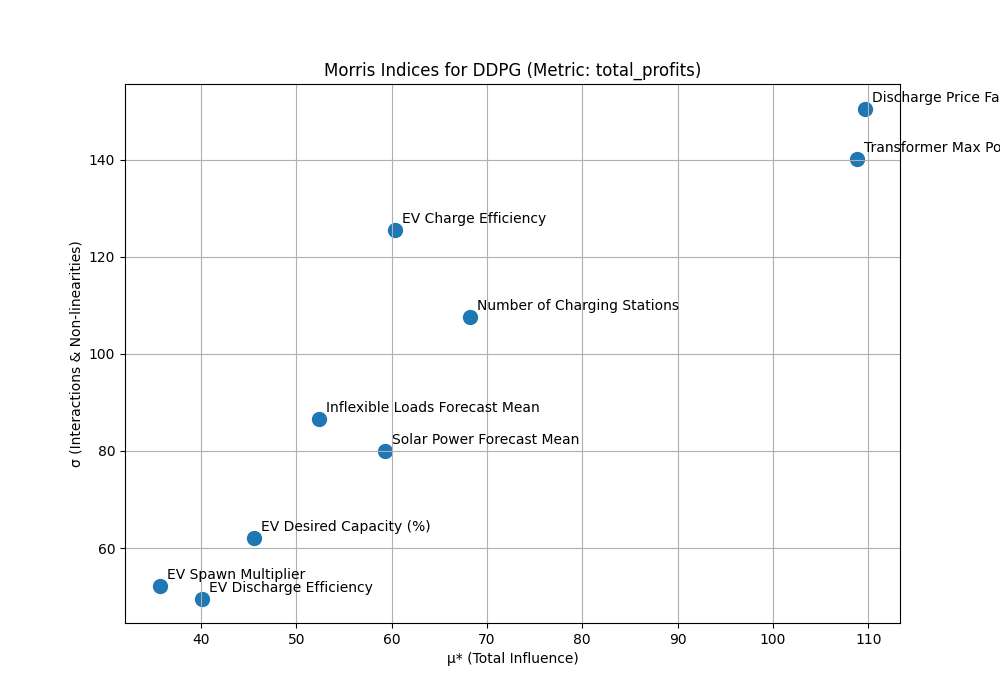
\includegraphics[width=\linewidth]{../sensitivity_analysis_results/Morris_20251021_091828/morris_plot_DDPG.png}
        \caption{Morris Analysis for DDPG}
        \label{fig:morris_ddpg}
    \end{subfigure}
    \hfill
    \begin{subfigure}{0.49\textwidth}
        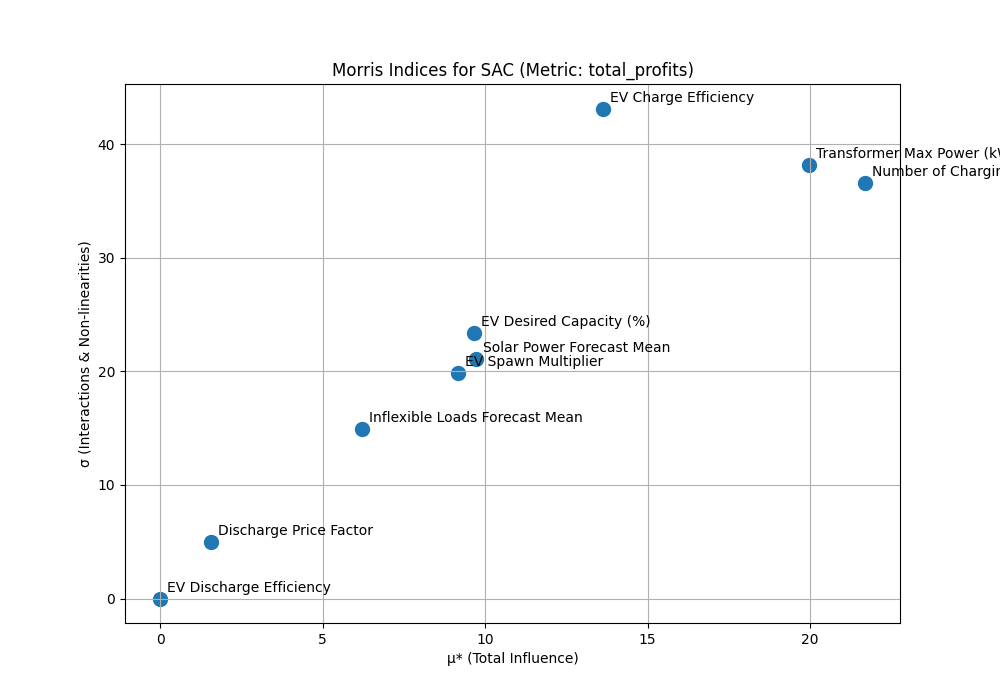
\includegraphics[width=\linewidth]{../sensitivity_analysis_results/Morris_20251021_211648/morris_plot_SAC.png}
        \caption{Morris Analysis for SAC}
        \label{fig:morris_sac}
    \end{subfigure}
    \caption{Morris sensitivity analysis plots for DDPG and SAC. The comparison reveals both shared sensitivities and critical differences in their learned strategies.}
    \label{fig:morris_plots_comparison}
\end{figure}

\subsubsection{Critical Interpretation and Comparison}

A detailed examination of the plots in Figure \ref{fig:morris_plots_comparison} reveals key differences in what each agent learned to prioritize.

\begin{itemize}
    \item \textbf{Shared Dominant Factor:} For both DDPG and SAC, the \textbf{Transformer Max Power} stands out with a very high mean effect ($\mu^*$) and a high standard deviation ($\sigma$). This is an expected and reassuring result, confirming that both agents correctly identified the Trasformer Power as a key element to consider.

    \item \textbf{Divergence in Secondary Factors:} The most interesting insights come from the secondary parameters. For the \textbf{DDPG} agent, the \textbf{Discarge price factor} is the next most influential parameters. This suggests that DDPG's deterministic policy is highly focused on price spread.

    \item In stark contrast, the \textbf{SAC} agent displays a high sensitivity to \textbf{EV Charge Efficiency} , \textbf{Number of Charging Stations} and Maximum Transformer Power (this last one is enforced by the OAT analysis see \ref{fig:oat_transformer_degradation_sac}) all of these have high $\mu^*$ and $\sigma$. The sensitivity to charge efficiency is particularly noteworthy and was not observed in the DDPG agent. This suggests that SAC's stochastic and more exploratory policy learns to exploit the subtle, non-linear effects of charging efficiency, perhaps by identifying specific conditions where small efficiency gains lead to disproportionately large profit increases.
\end{itemize}

\subsection{One-at-a-Time (OaaT) Results}
The OaaT analysis further clarifies the direct relationships between key parameters and system outputs.



\begin{figure}[H]
    \centering
    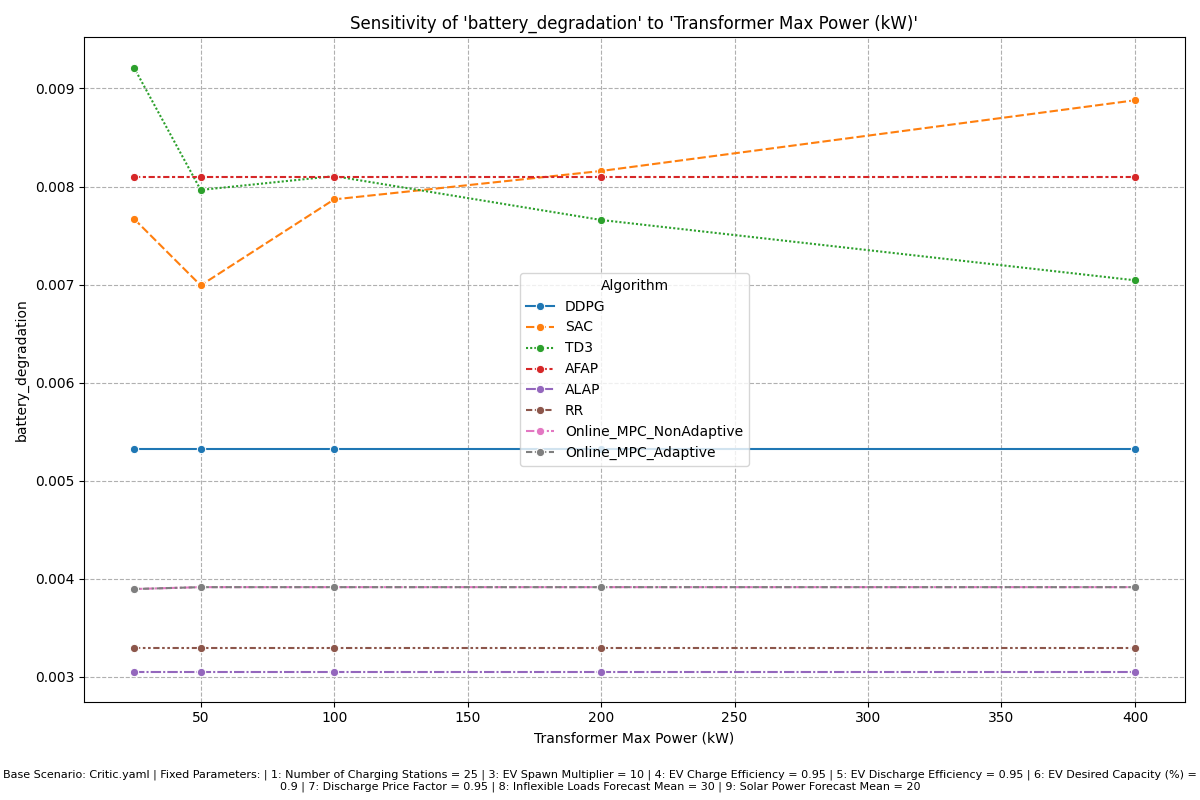
\includegraphics[width=0.8\linewidth]{../sensitivity_analysis_results/Risultati_scelti/sensitivity_Transformer_Max_Power_(kW)_vs_battery_degradation.png}
    \caption{Impact of maximum transformer power on battery degradation for the SAC algorithm.}
    \label{fig:oat_transformer_degradation_sac}
\end{figure}
\noindent
Figure \ref{fig:oat_transformer_degradation_sac} provides further confirmation of the significant influence of \textbf{Maximum Transformer Power} on battery degradation for the SAC agent, as identified by Morris' analysis.  This highlights how adequate transformer sizing is crucial to mitigate battery degradation and optimize the useful life of SAC-managed EVs.





\begin{figure}[H]
    \centering
    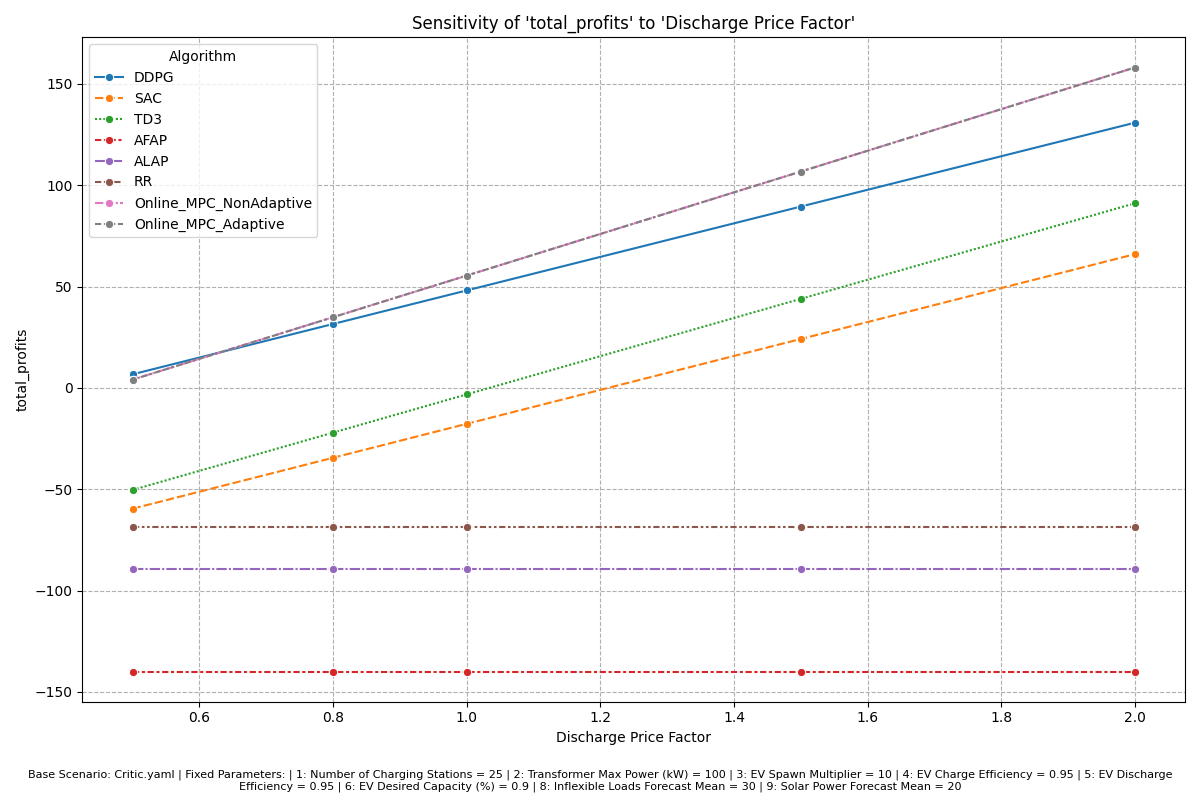
\includegraphics[width=0.8\linewidth]{../sensitivity_analysis_results/Risultati_scelti/sensitivity_Discharge_Price_Factor_vs_total_profits.png}
    \caption{Impact of Discharge Price Factor on Total Profits for various algorithms.}
    \label{fig:oat_discharge_profit}
\end{figure}

As shown in Figure \ref{fig:oat_discharge_profit}, for all V2G-capable algorithms (SAC, DDPG, MPC), profit increases substantially as the \textbf{Discharge Price Factor} rises above 1.0. This confirms the finding from the Morris analysis that this is the most critical economic lever. Heuristic algorithms that do not discharge (AFAP, ALAP) are, as expected, unaffected.

\begin{figure}[H]
    \centering
    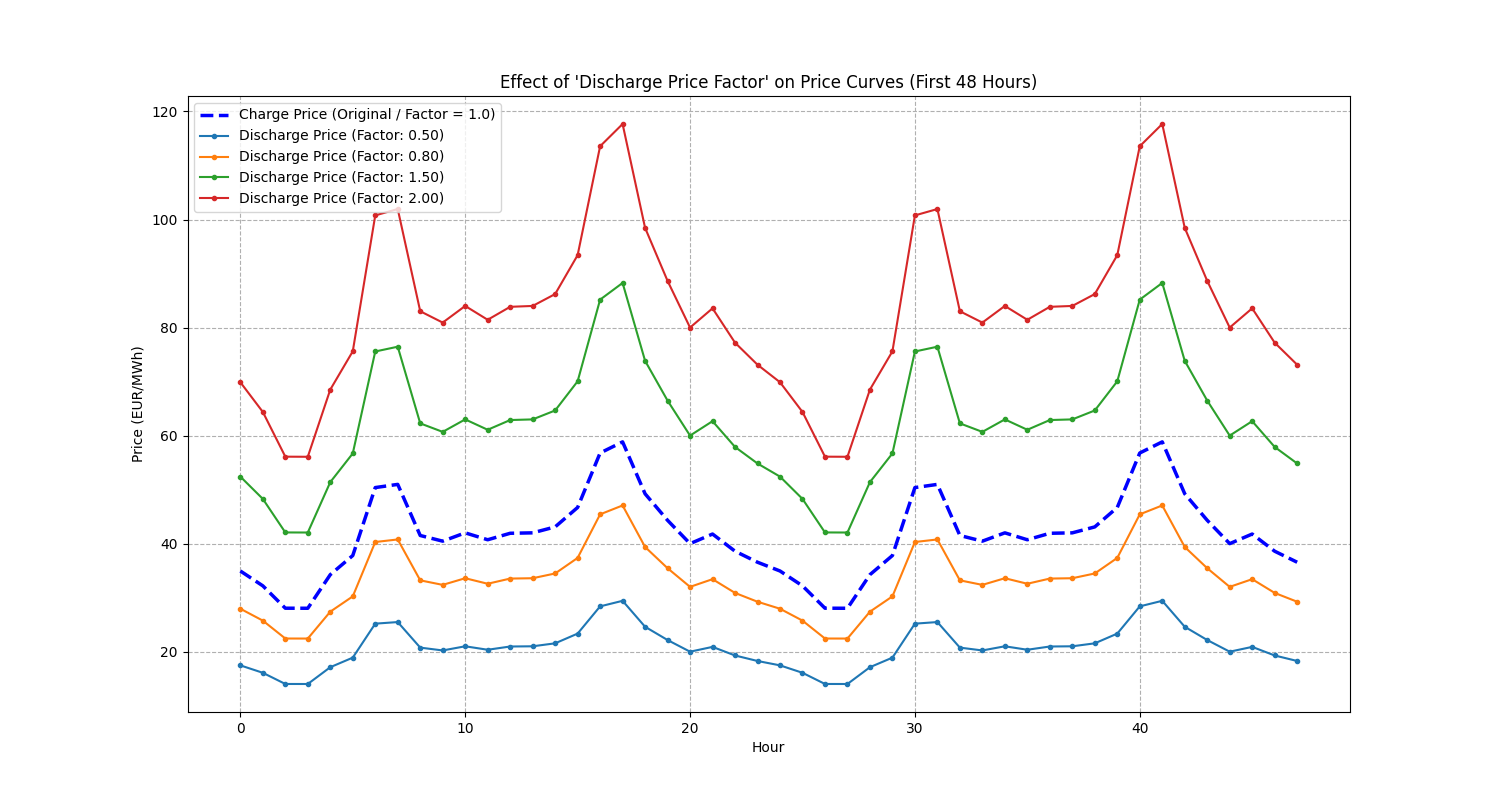
\includegraphics[width=0.8\linewidth]{../sensitivity_analysis_results/Risultati_scelti/price_curves_vs_discharge_factor.png}
    \caption{Illustration of how the discharge price (selling price) changes relative to the charge price (buying price) based on the discharge price factor.}
\end{figure}
\noindent
Figure \ref{fig:price_curves} provides a visual explanation for the results in the previous plot, showing how a factor greater than 1.0 makes the selling price consistently higher than the buying price, creating clear arbitrage opportunities.

\begin{figure}[H]
    \centering
    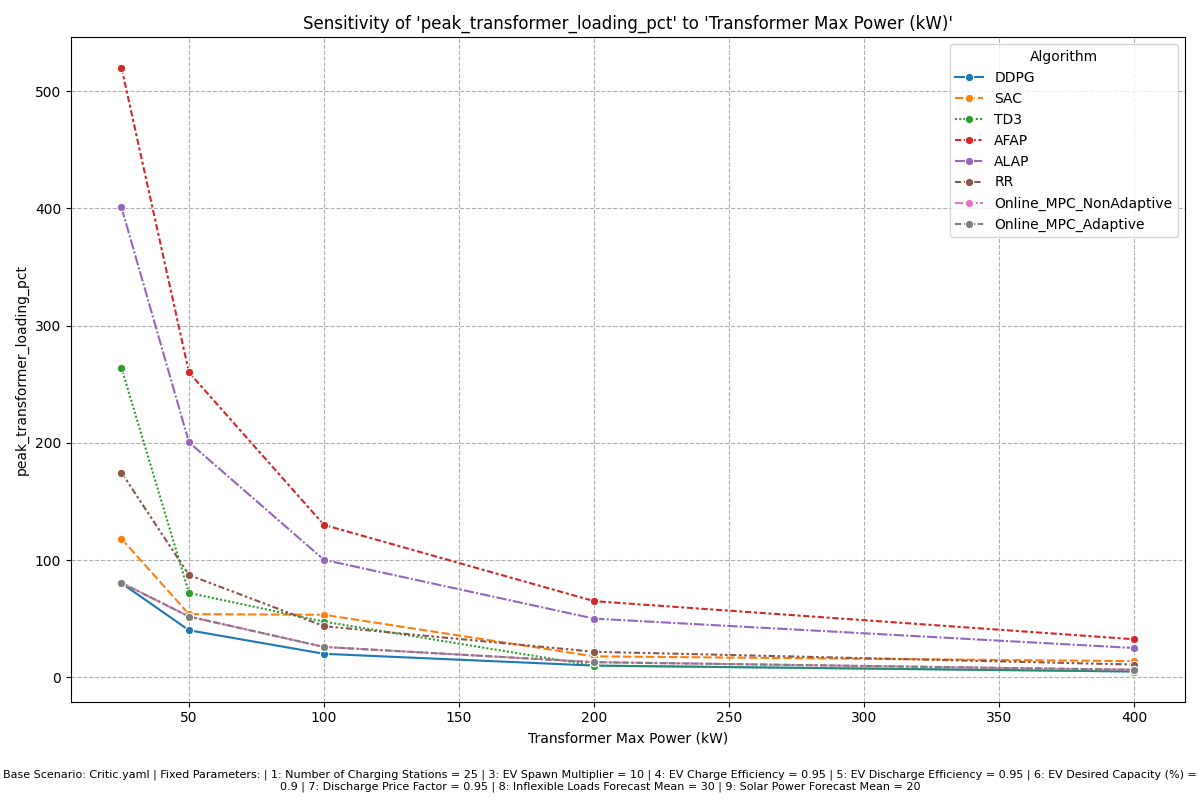
\includegraphics[width=0.8\linewidth]{../sensitivity_analysis_results/Risultati_scelti/sensitivity_Transformer_Max_Power_(kW)_vs_peak_transformer_loading_pct.png}
    \caption{Impact of Transformer Max Power on Peak Transformer Loading.}
    \label{fig:oat_transformer_load}
\end{figure}
\noindent
Figure \ref{fig:oat_transformer_load} illustrates the direct impact of transformer capacity on grid stress. For unintelligent algorithms like AFAP, peak loading remains dangerously high until the transformer capacity is significantly oversized. In contrast, proactive controllers like DDPG, and MPC adapt their behavior to respect the transformer's limit, keeping peak load consistently below 100\% across a wide range of capacities. This demonstrates their crucial role in maintaining grid stability.However TD3 shows that without proper optimization cannot go well then DDPG even though it's a DDPG improvement.

\begin{figure}[H]
    \centering
    \includegraphics[width=0.8\linewidth]{\detokenize{../sensitivity_analysis_results/Risultati_scelti/sensitivity_EV_Desired_Capacity_(\%)_vs_average_user_satisfaction.png}}
    \caption{Impact of EV Desired Capacity on Average User Satisfaction.}
    \label{fig:oat_desired_capacity}
\end{figure}
\\
\noindent
Figure \ref{fig:oat_desired_capacity} shows that as the users' desired state of charge increases, it becomes more challenging for all algorithms to achieve high satisfaction. Notably, heuristic algorithms like AFAP and ALAP maintain near-perfect satisfaction as they have a singular focus on charging, whereas the more intelligent agents must balance this goal against others like profit maximization and grid stability.

\subsection{Reward Function and Curriculum Learning Analysis}
A key contribution of this work was the development of the \textbf{FastProfitAdaptiveReward} function and a Curriculum Learning (CL) strategy to improve agent training.

\begin{figure}[H]
    \centering
    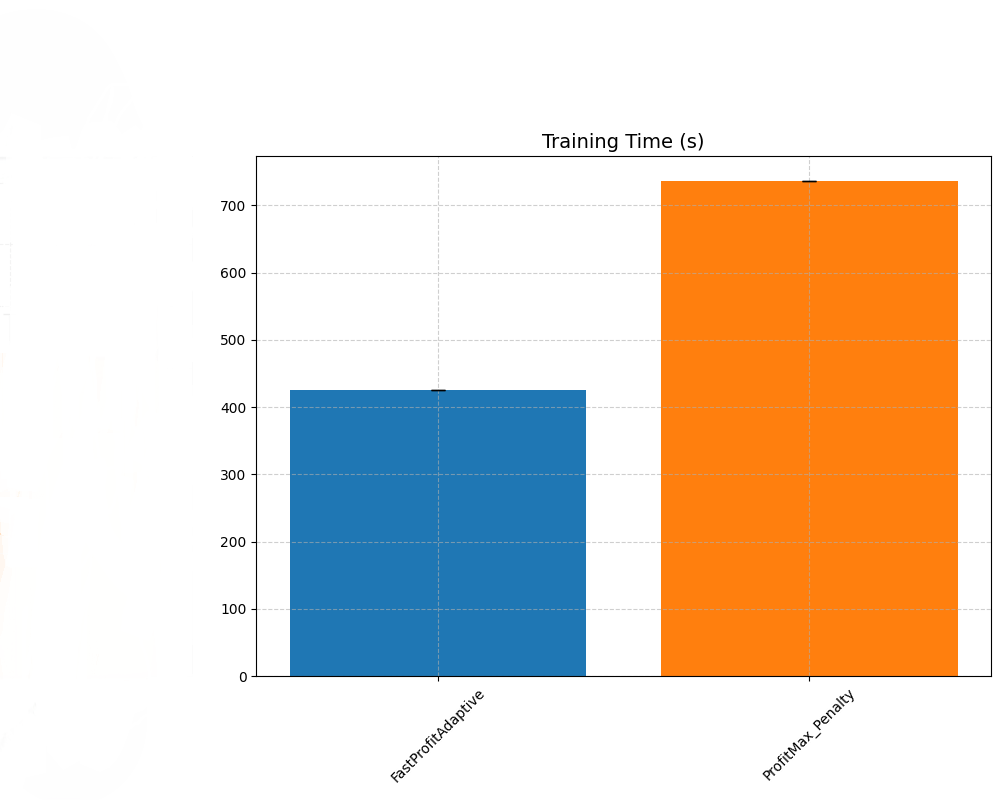
\includegraphics[width=0.5\textwidth]{../sensitivity_analysis_results/Risultati_scelti/performance_summary_RewardFunctionComparison.png}
    \caption{Training time performance comparison between the original reward function (\textbf{ProfitMax\_Penalty}) and the new adaptive function (\textbf{FastProfitAdaptive}), with and without Curriculum Learning.}
    \label{fig:reward_comparison_summary}
\end{figure}

\begin{figure}[H]
    \centering
    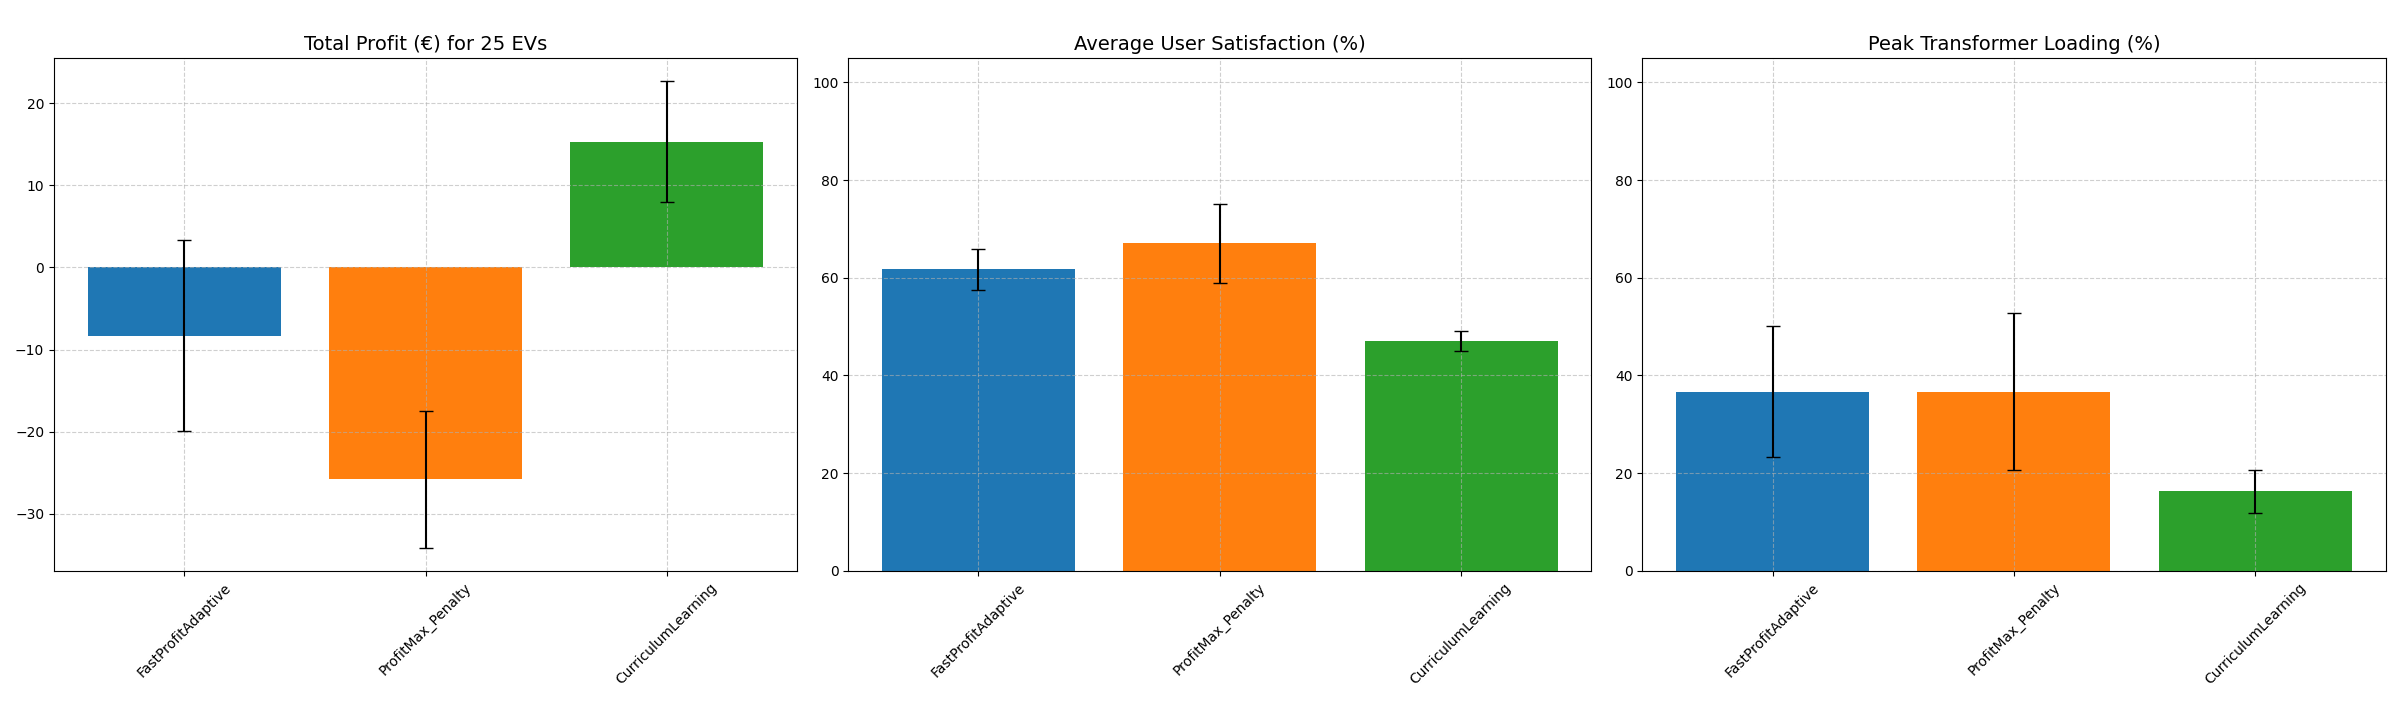
\includegraphics[width=0.7\textwidth]{../sensitivity_analysis_results/Risultati_scelti/RewardFunctionComparison_profit.png}
    \caption{Performance comparison on the KPI between the original reward function (\textbf{ProfitMax\_Penalty}) and the new adaptive function (\textbf{FastProfitAdaptive}), with and without Curriculum Learning.}
    \label{fig:reward_comparison_summary_2}
\end{figure}
\noindent
As summarized in Figure \ref{fig:reward_comparison_summary_2}, the DDPG agent trained with the CL method significantly outperforms the one trained with the original, achieving higher profits and better overall performance because it uses both the advantage of the two reward funtions.
\begin{figure}[H]
    \centering
    \begin{subfigure}{0.49\textwidth}
        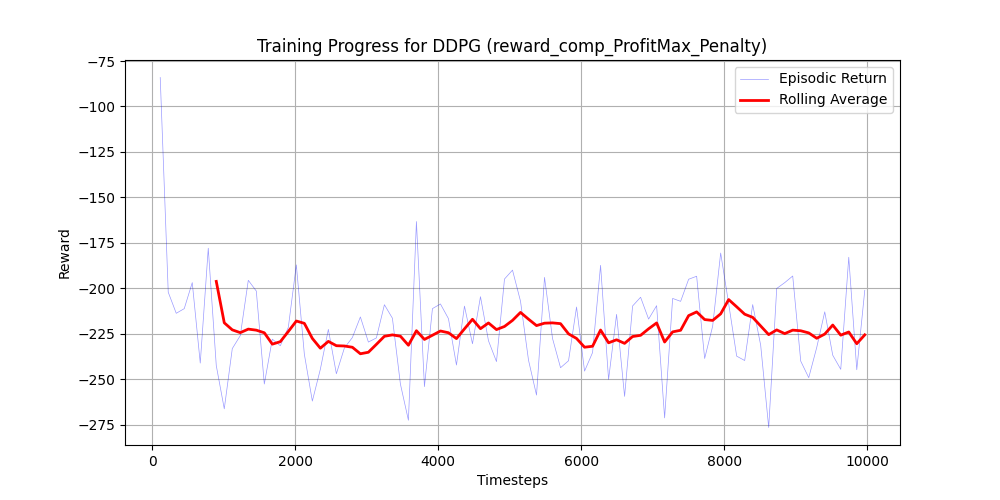
\includegraphics[width=\linewidth]{../sensitivity_analysis_results/Risultati_scelti/DDPG_reward_comp_ProfitMax_Penalty_20251022_084014.png}
        \caption{Original Reward}
    \end{subfigure}
    \hfill
    \begin{subfigure}{0.49\textwidth}
        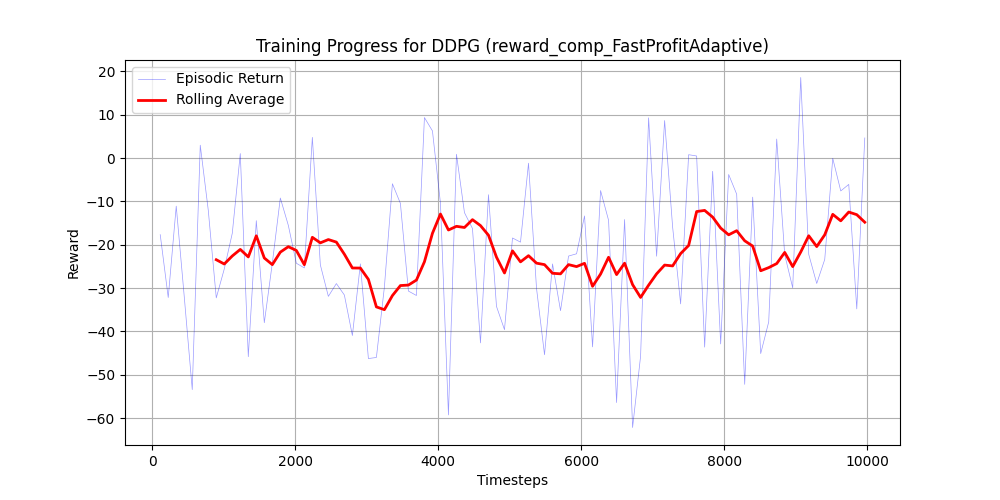
\includegraphics[width=\linewidth]{../sensitivity_analysis_results/Risultati_scelti/DDPG_reward_comp_FastProfitAdaptive_20251022_083514.png}
        \caption{New Adaptive Reward}
    \end{subfigure}
    \caption{Comparison of training progress for DDPG with the original vs. the new adaptive reward function. The new function leads to a more stable and consistently positive reward signal during training.}
    \label{fig:ddpg_rewards}
\end{figure}

\subsubsection{Curriculum Learning Stages}
The CL strategy involved two stages:
\begin{enumerate}
    \item \textbf{Stage 1 (First 5000 steps):} The agent is trained with the original \textbf{ProfitMax\_Penalty} reward, forcing it to first learn basic constraint satisfaction.
    \item \textbf{Stage 2 (After 5000 steps):} The reward function switches to the new \textbf{FastProfitAdaptiveReward}, encouraging the agent to build upon its foundation of safe behavior to explore more profitable strategies.
\end{enumerate}

\begin{figure}[H]
    \centering
    \begin{subfigure}{0.49\textwidth}
        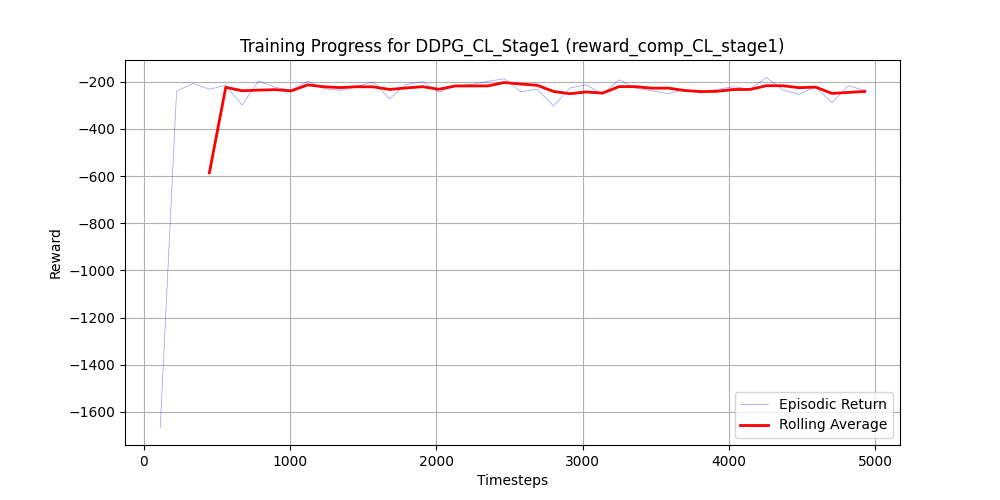
\includegraphics[width=\linewidth]{../sensitivity_analysis_results/Risultati_scelti/DDPG_CL_Stage1_reward_comp_CL_stage1_20251022_084237.png}
        \caption{CL Stage 1: Learning basic constraints.}
    \end{subfigure}
    \hfill
    \begin{subfigure}{0.49\textwidth}
        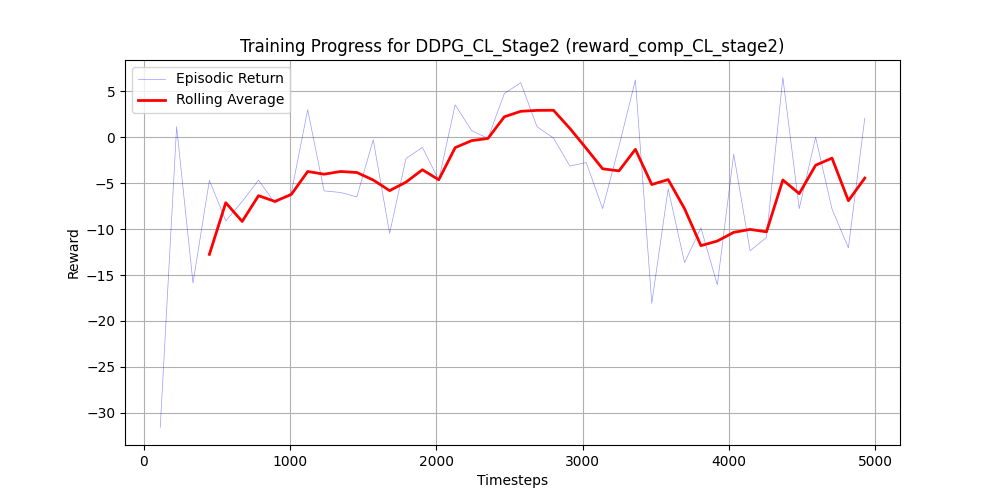
\includegraphics[width=\linewidth]{../sensitivity_analysis_results/Risultati_scelti/DDPG_CL_Stage2_reward_comp_CL_stage2_20251022_084506.png}
        \caption{CL Stage 2: Optimizing for profit.}
    \end{subfigure}
    \caption{Training progress during the two stages of Curriculum Learning. A clear and significant improvement in reward is visible upon switching to the adaptive reward function in Stage 2, demonstrating the effectiveness of the CL strategy.}
    \label{fig:cl_stages}
\end{figure}

Figure \ref{fig:cl_stages} clearly shows the success of this approach. In Stage 2, the agent's reward immediately and consistently climbs to a much higher level than what was achievable with either reward function alone. This confirms that by first establishing a baseline of safe behavior and then optimizing for profit, the CL strategy enables the agent to discover superior policies.



\section{Conclusion}
The sensitivity analysis performed in this chapter provides critical insights into the dynamics of the V2G control problem. The results clearly indicate that the system's performance is not equally sensitive to all parameters. Economic factors, such as the \textbf{Discharge Price Factor}, and hard physical constraints, like the \textbf{Transformer Max Power}, were identified as the most dominant drivers of profitability and grid stability.
\noindent
The analysis also highlighted the different responses of various control strategies to these parameter changes. While simple heuristics are brittle and perform poorly outside of their optimal operating conditions, advanced controllers like MPC and RL agents demonstrate greater resilience, although their performance is still heavily influenced by these key parameters.
\noindent
These findings have significant implications for the development of robust control agents. A successful generalist agent must be able to recognize the current parameter regime (e.g., a low-price-spread environment vs. a high-spread one) and adapt its strategy accordingly. The insights gained from this analysis directly inform the design of the reward functions and state representations for the reinforcement learning agents developed in the subsequent chapters.
